\documentclass{article}
\usepackage[utf8]{inputenc}

\title{Análisis Exploratorio de Datos \\ Trabajo Práctico 1 - Organización de Datos}
\author{Nombre de grupo}
\date{Poner fecha}

\usepackage{natbib}
\usepackage{graphicx}
\newcommand\tab[1][1cm]{\hspace*{#1}}
\usepackage{placeins}

\begin{document}
\begin{figure}
    \centering
    \makebox[\textwidth]{
\includegraphics[width=250pt]{logofiuba.jpg}}
\end{figure}

\maketitle

\FloatBarrier
\begin{center}
        \begin{tabular}{ |c|c|c| }
          \hline
          Nombre & Padrón & Mail \\
          \hline\hline
          Álvarez, Federico & 99266 & fede.alvarez1997@gmail.com \\
          \hline
          La Torre, Gabriel & 87796 & latorregab@gmail.com \\
          \hline
          Medrano, Lucas Nicolás & 99247 & lucasmedrano97@gmail.com \\
          \hline
          Piro Martino, Ariel & 99469 & ariel.piro@hotmail.com \\
          \hline
        \end{tabular}
\end{center}
\FloatBarrier

\newpage

\tableofcontents
\newpage
\section{Introduction}
	\tab En el trabajo se hace un análisis exploratorio de un set de datos provistos por la empresa Jampp. En el mismo se encuentra información de subastas, instalaciones, clicks, entre otros.\\
	\tab Primero se hará una visión general de los archivos (installs.csv, clicks.csv, auctions.csv, events.csv) para entender la distribución y la cantidad de datos, el significado de las columnas, reconocer las columnas que no aportan información (por ejemplo, las que tienen todos sus valores nulos), reconocer el tipo de datos en cada columna, seguido de un análisis mas profundo para obtener mas información de los datos. Luego se hará un análisis global, buscando información relativa a los archivos en conjunto, permitiendo obtener otro tipo de información.

\section{Análisis individual de archivos}
\subsection{Subastas}
	\subsubsection{Análisis general}
	 \tab El archivo 'auctions.csv' contiene información acerca de subastas.
	Hay dos columnas que no nos aportan información significante. 'auction\_type\_id' tiene todos sus valores 		nulos, por lo que no fue tomada en cuenta para el análisis. 'country' informa un solo valor posible, que se supone que debe ser Argentina.
	\tab La columna platforms tiene dos valores posibles (1 y 2) que se supone son Android e iOS. Va a ser importante para el análisis que hagamos más adelante. De ahora en más, platform y sistema operativo serán sinónimos en este informe.
	\tab Por último, 'source' nos da información acerca del exchange de donde surge la subasta.
	\tab Además vemos que ningún valor de este archivo, excluyendo la columna 'auction\_type\_id', es nulo, por lo que no es necesario tomar ninguna decisión respecto a eso.
	
	\subsubsection{Subastas por día de Marzo}
	\tab Como primer acercamiento a este set de datos, es interesante ver cómo se distribuye la cantidad de subastas en los días que incluye el archivo (05/03/19 al 13/03/19). El gráfico \ref{subastasmarzo} representa dicha distribución. En él se pueden observar varias cosas:
	\begin{itemize}
		\item La cantidad de subastas parece, en general, aumentar con el paso de los dias.
		\item El valor del último día es mas del doble del valor del primer día.
		\item El mayor aumento se da del sexto al septimo día.
		\item La cantidad de subastas varía entre unos valores extremos, aproximados, de un millón y 3 millones.
	\end{itemize}
	\FloatBarrier
		\begin{figure}
			\centering
			   	\makebox[\textwidth]{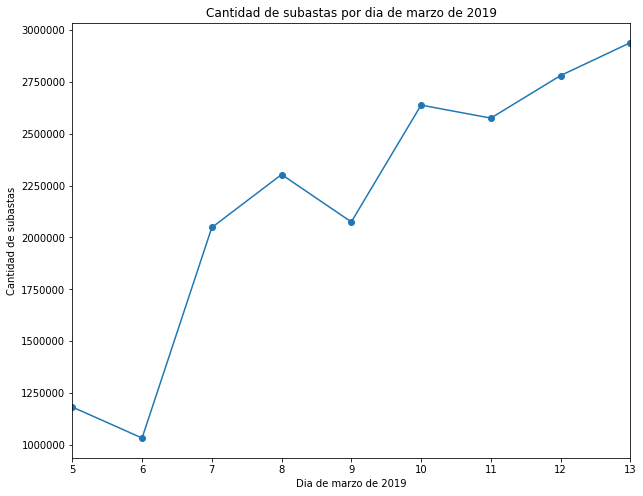
\includegraphics[width=300pt]{images/auctions/subastaspordia.png}}
		   		\caption{Cantidad de subastas por día de Marzo}
			   	\label{subastasmarzo}
		\end{figure}
	\FloatBarrier
			
	\subsubsection{Subastas por día de Marzo por sistema operativo}
	\tab Otro punto interesante es dividir el problema. Obtener la distribución de subastas en los días con datos disponibles para cada plataforma (Android e iOS). En la imagen \ref{subastasmarzoSO} se pueden observar las cantidades. Observese que llamamos '1' y '2' a las plataformas, ya que no sabemos cuál es Android y cuál es iOS.
	\tab Puntos interesantes a reconocer:
	
	\begin{itemize}
		\item La cantidad de subastas para la plataforma '1' es, salvo en el cuarto y el quinto día, considerablemente mayor a la cantidad para la plataforma '2'.
		\item La figura de la plataforma '2' es mucho mas "chata" que la de la plataforma '1', la cual representa mas picos y saltos.
		\item La figura de la plataforma '1' es muy parecida a la del gráfico \ref{subastasmarzo}, mientras que la de la plataforma '2' no lo es. Esto es resultado, principalmente, de lo indicado en el primer ítem. Este análisis puede llegar a ser muy útil para reconocer partes de los datos que son representativas del total.
	\end{itemize}
	\FloatBarrier
		\begin{figure}
			\centering
	   		\makebox[\textwidth]{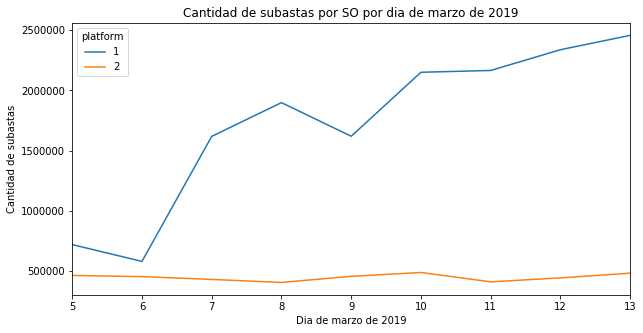
\includegraphics[width=350pt]{images/auctions/subastaspordiaSO.png}}
		   	\caption{Cantidad de subastas por día de Marzo y por sistema operativo}
		   	\label{subastasmarzoSO}
		\end{figure}
	\FloatBarrier
			
	\subsubsection{Subastas por hora del día}
	\tab Ahora vamos a analizar cómo se distribuyen las subastas a lo largo del día. Para esto hacemos un gráfico de hora del día contra cantidad de subastas (Gráfico \ref{subastashora}).\newline
	\tab Desde un análisis cualitativo se pueden observar algunos puntos:
	\begin{itemize}
		\item Parece ser que la mayor cantidad de subastas se distribuyen por la noche y la madrugada.
		\item La cantidad de subastas es poca en horas de la mañana y el mediodía. En el gráfico se puede ver un gran valle en esa parte del día.
		\item 
	\end{itemize}
	
	\FloatBarrier
		\begin{figure}
			\centering
			\makebox[\textwidth]{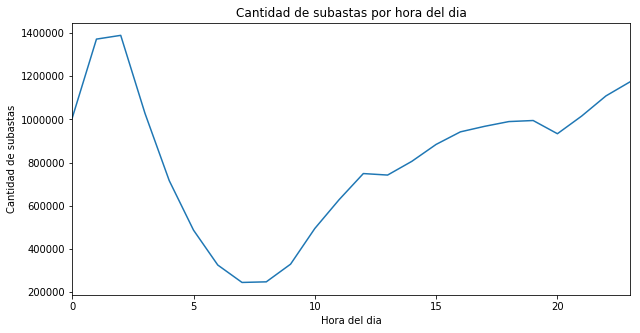
\includegraphics[width=350pt]{images/auctions/subastasporhora.png}}
		   	\caption{Subastas por día de Marzo}
			\label{subastashora}
		\end{figure}
	\FloatBarrier
	\subsubsection{Subastas por día por sistema operativo}
	\subsubsection{Subastas por sistema operativo}
	\subsubsection{Subastas por source}
	

\subsection{Clicks}

\subsection{Eventos}

\subsection{Instalaciones}
	\subsubsection{Introducción}
		Los datos sobre instalaciones fueron provistos por Jampp en el archivo \texttt{installs.csv}, el cual contenía información acerca de todas las instalaciones registradas entre los días 5 y 13  Marzo del corriente año, indicando el tipo de aplicaciones descargadas, su fecha de descarga, país de origen, modelo, marca e idioma del dispositivo, entre otras cosas. 
	
		Cabe destacar que se descartaron datos como las direcciones ip y los varios id únicos generados para cada instalación, puesto que no aportaban información relevante al análisis que se pretende hacer en este trabajo, como también los datos del \textit{session user agent}, ya que la misma empresa informó que no los consideran de importancia y pudieron haberse visto modificados por los propios agentes que les proveyeron los datos.
	
	\subsubsection{Instalaciones por día y hora}
		Para comenzar, lo primero que haremos será ver cómo se distribuyen las instalaciones en el periodo dado. 
		\FloatBarrier
		\begin{figure}
			\centering
			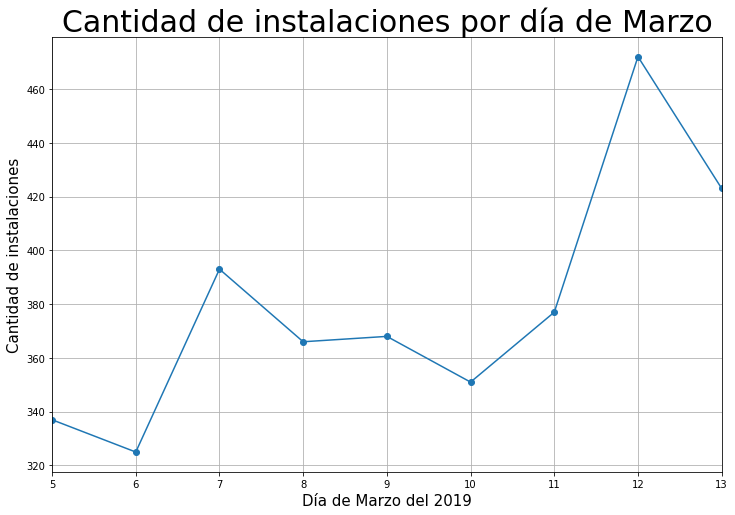
\includegraphics[width=350pt]{images/installs/installspordia.png}
			\caption{Instalaciones por día de Marzo}
		\end{figure}
		\FloatBarrier
		
		Como se puede observar, se registran ascensos considerables entre los días 6 y 7 y 11 y 12, con respectivas caídas al día siguiente, pero manteniendo una tendencia general al alza.
		
		\FloatBarrier
		\begin{figure}
			\centering
			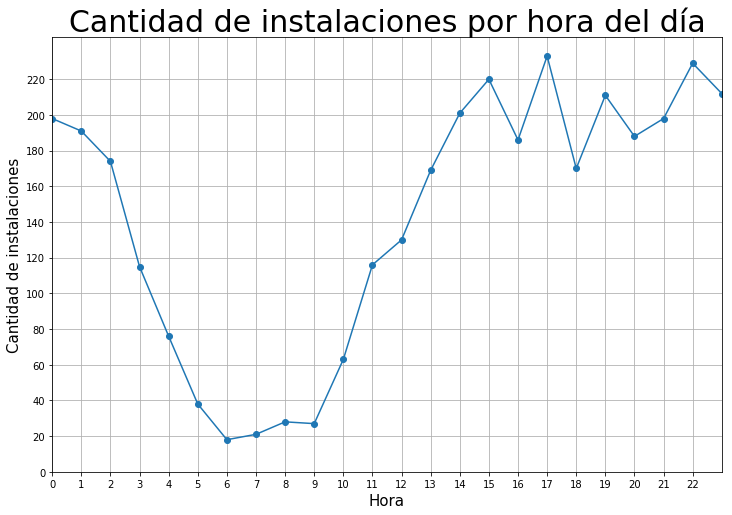
\includegraphics[width=350pt]{images/installs/installsxhora.png}
			\caption{Instalaciones por hora del día}
		\end{figure}
		\FloatBarrier
		
		 El gráfico anterior nos indica que la gran mayoría de las instalaciones se registran en horas de la tarde y la noche, con un pico a las 5 de la tarde. Cabe destacar a su vez el notorio valle que se da en horas de la mañana, donde el número es hasta diez veces menor que en el punto máximo.
		 
		 Para un análisis más general, la siguiente figura engloba los dos puntos mencionados anteriormente.
		 
		\FloatBarrier
		\begin{figure}
			\centering
			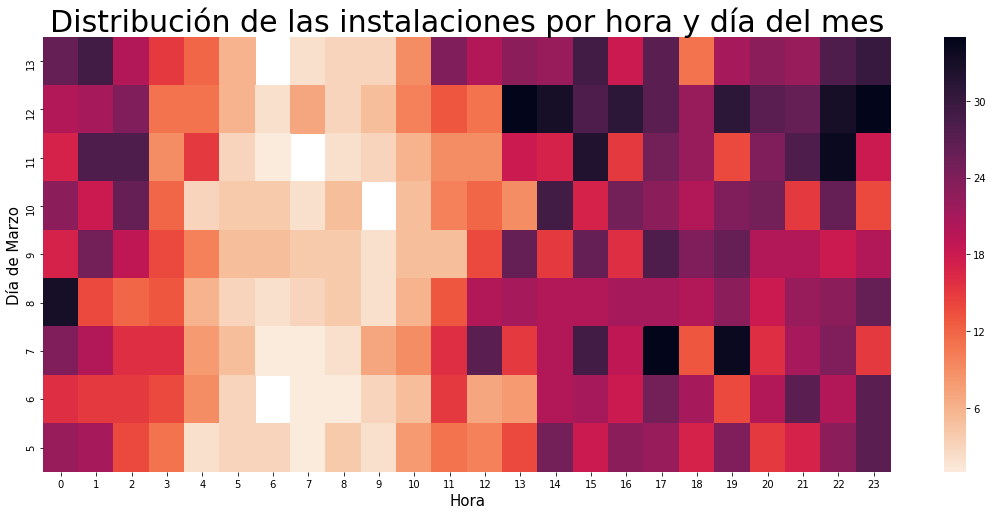
\includegraphics[width=350pt]{images/installs/heatmapfecha.png}
			\caption{Instalaciones por fecha y hora}
		\end{figure}
		\FloatBarrier
		
		Se puede observar claramente el valle de las horas de la mañana, como así también el pico que se da en el día 12. Sin embargo, este gráfico resulta útil ya que permite notar que tanto en los días 6 y 13 a las 6 de la mañana, el día 11 a las 7 y el 10 a las 9 no se produjo ninguna instalación.
		
	\subsubsection{Instalaciones por aplicación}
		Resultará de utilidad conocer de que aplicación provienen las instalaciones registradas y observar cual es la tendencia en ese aspecto.
		
		\FloatBarrier
		\begin{figure}
			\centering
			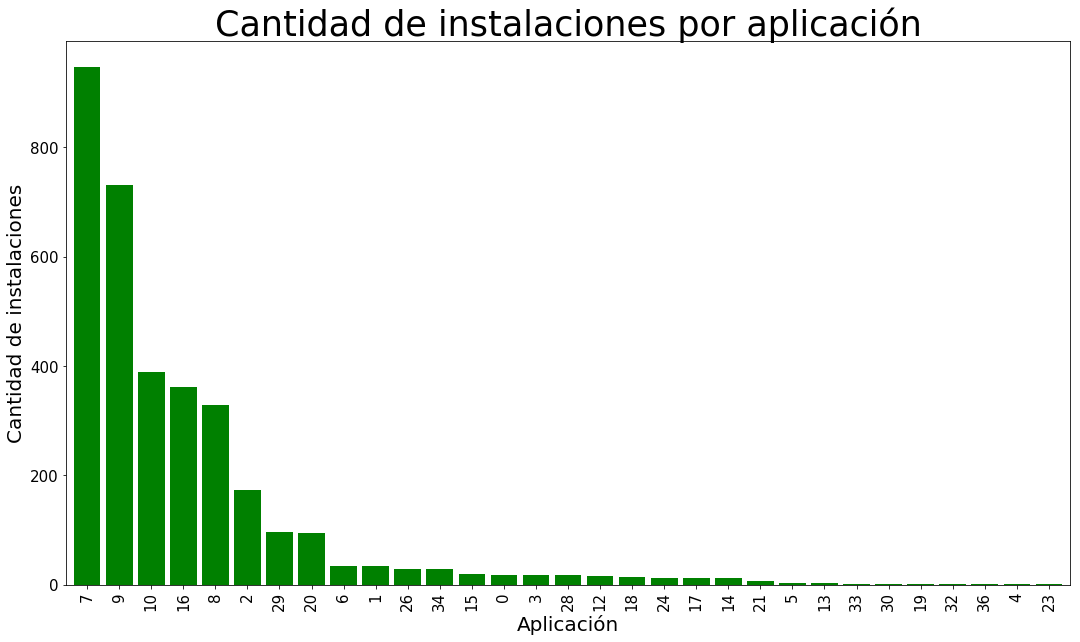
\includegraphics[width=350pt]{images/installs/aplicacionesvc.png}
			\caption{Instalaciones por aplicación}
		\end{figure}
		\FloatBarrier
		
		La figura anterior muestra un dominio claro de las aplicaciones 7 y 9 por sobre las demás, ya que la segunda casi duplica en cantidad a la tercera. Además, se puede ver otra diferencia importante{\textemdash}otra vez, de casi el doble{\textemdash}entre la quinta y la sexta, lo que deja en evidencia cuales son las que dominan en este campo, puesto que las primeras cinco aplicaciones concentran más del 80\% de las instalaciones.
		
	\subsubsection{Instalaciones por fecha según la aplicación}
		A continuación veremos a qué aplicaciones pertenecen las instalaciones según el día y la hora del día, lo que puede servir para determinar en qué momento apostar por una u otra aplicación. Cabe destacar que, para ello se agruparon todas aquellas aplicaciones que generaron un número muy bajo (menos de 90) de instalaciones en la categoría \textit{other}.
		
		\FloatBarrier
		\begin{figure}
			\centering
			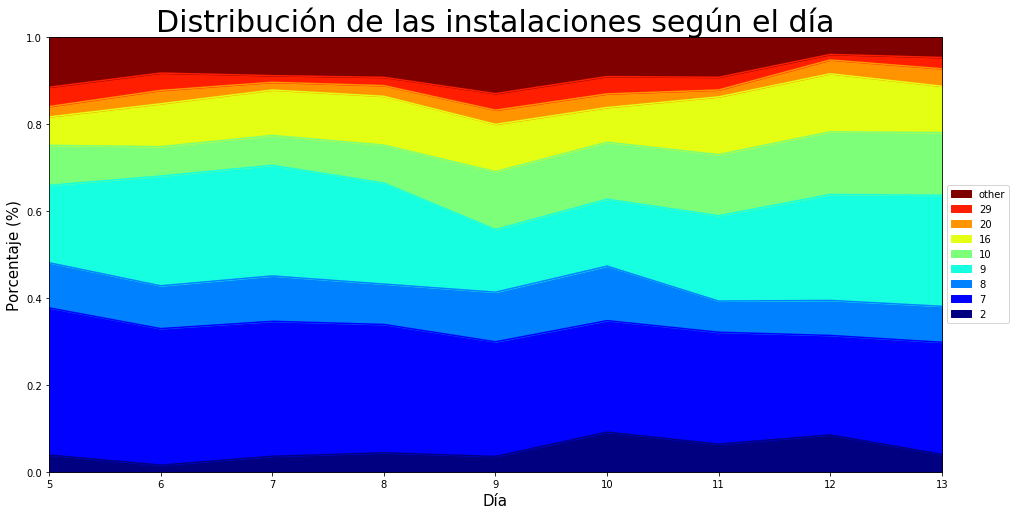
\includegraphics[width=350pt]{images/installs/appsxdiaarea.png}
			\caption{Incidencia de las aplicaciones según el día}
		\end{figure}
		\FloatBarrier
		
		Como se puede observar, la aplicación 7 dominó la mayoría de los días aunque disminuyendo hacia el 12 y el 13, donde fue superada por la 9. La tercera aplicación con más instalaciones, la 10, se mantuvo bastante estable durante los últimos cinco días, mientras que los días 10 y 12 la número 2, de poca preponderancia en otros días, obtuvo su mejor resultado. Cabe aclarar además, que si bien en días como el 9 se ve bastante incidencia de la categoría \textit{other}, ésta engloba los resultados de 23 aplicaciones distintas.
		
		\FloatBarrier
		\begin{figure}
			\centering
			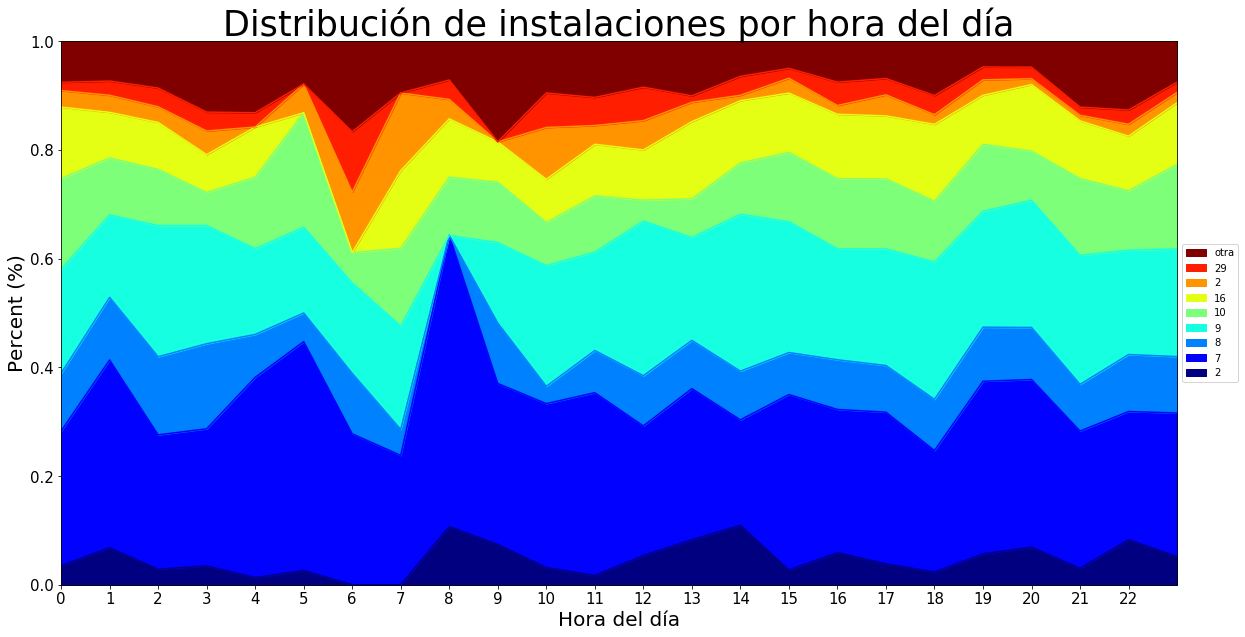
\includegraphics[width=350pt]{images/installs/appsxhora.png}
			\caption{Incidencia de las aplicaciones según la hora del día}
		\end{figure}
		\FloatBarrier
		
		En cuanto a la hora cabe destacar que la segunda aplicación en instalaciones no tiene presencia alguna a las 8 a.m., que es a su vez el momento del día donde más incidencia tiene una aplicación de poca presencia como la 2. La tendencia sigue mostrando a la número 7 como dominadora absoluta en todos los horarios.
		
		
\section{Análisis de archivos en conjunto}

\section{Conclusion}


\bibliographystyle{plain}
\bibliography{references}
\end{document}
